% SC3000 — Chapter 4: Constraint Satisfaction Problems (0->100)
% No \documentclass — included by main.tex
\chapter{Constraint Satisfaction Problems}
\label{ch:csp}

\begin{quote}
\emph{``Search with structure.''} A CSP separates \emph{what} must hold (constraints) from \emph{how} we search, so generic propagation plus backtracking solves map-colouring, scheduling, and Sudoku with the same engine.
\end{quote}

\noindent\fbox{\parbox{\dimexpr\linewidth-2\fboxsep-2\fboxrule}{%
\textbf{From zero: states $\to$ constraints.} We assume only state-space search from Ch.~2--3 and build CSPs from scratch: variables, domains, and relations before any algorithm. No prior logic or graph theory beyond sets.}}
\vspace{0.4em}

\section*{Learning Outcomes}
After this chapter you will be able to:
\begin{enumerate}[label=(L\arabic*)]
    \item formalise a problem as a CSP $(V,D,C)$ and draw its constraint graph;
    \item trace backtracking search with MRV, degree, and LCV heuristics;
    \item apply forward checking to prune domains and detect early failure;
    \item define arc consistency and execute AC-3 step by step;
    \item compare backtracking, FC, and MAC (backtracking+AC-3) trade-offs.
\end{enumerate}

% ============================================================
\section{CSP Formalism and Constraint Graphs}
\label{sec:csp-formal}

\begin{definition}[CSP]
A \emph{constraint satisfaction problem} is a triple $(V,D,C)$ where $V=\{X_1,\dots,X_n\}$ are variables, each $X_i$ has domain $D_i$ (finite), and $C$ is a set of constraints. Each $c\in C$ has scope $\mathrm{scope}(c)\subseteq V$ and relation $\mathrm{rel}(c)\subseteq\prod_{X_i\in\mathrm{scope}(c)} D_i$ of allowed tuples. A \emph{solution} assigns $x_i\in D_i$ to every $X_i$ satisfying all $c$.
\end{definition}

Unary constraints involve one variable ($X\neq$~red), binary involve two ($X\neq Y$), global involve many (AllDifferent). Binary CSPs suffice in theory (auxiliary variables reduce higher arities) and dominate practice.

\begin{example}[Australia map-colouring]
Variables $V=\{\mathrm{WA},\mathrm{NT},\mathrm{SA},\mathrm{Q},\mathrm{NSW},\mathrm{V},\mathrm{T}\}$, $D_i=\{r,g,b\}$, constraints $X\neq Y$ for adjacent regions. SA touches five neighbours, so it is most constrained---a fact heuristics will exploit.
\end{example}

The \emph{constraint graph} has a node per variable and an edge per binary constraint. It reveals structure: sparse graphs are easy to cut, dense or highly connected variables bottleneck search.

\begin{figure}[h!]
\centering
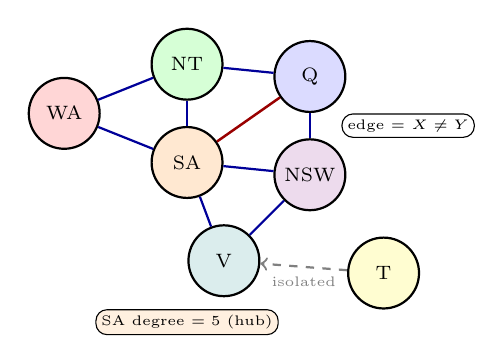
\begin{tikzpicture}[scale=0.78, every node/.style={font=\scriptsize},
  var/.style={circle, draw, thick, minimum size=0.9cm, inner sep=1pt}]
  \node[var, fill=red!16] (WA) at (0,1.4) {WA};
  \node[var, fill=green!16] (NT) at (2,2.2) {NT};
  \node[var, fill=orange!18] (SA) at (2,0.6) {SA};
  \node[var, fill=blue!14] (Q) at (4,2.0) {Q};
  \node[var, fill=violet!14] (NSW) at (4,0.4) {NSW};
  \node[var, fill=teal!14] (V) at (2.6,-1.0) {V};
  \node[var, fill=yellow!18] (T) at (5.2,-1.2) {T};
  \draw[thick, blue!60!black] (WA) -- (NT); \draw[thick, blue!60!black] (WA) -- (SA);
  \draw[thick, blue!60!black] (NT) -- (SA); \draw[thick, blue!60!black] (NT) -- (Q);
  \draw[thick, red!60!black, line width=0.9pt] (SA) -- (Q); \draw[thick, blue!60!black] (SA) -- (NSW);
  \draw[thick, blue!60!black] (SA) -- (V); \draw[thick, blue!60!black] (Q) -- (NSW);
  \draw[thick, blue!60!black] (NSW) -- (V);
  \node[font=\tiny, fill=orange!12, draw, rounded corners, inner sep=2pt, align=center] at (2,-2.0) {SA degree $=5$ (hub)};
  \node[font=\tiny, fill=white, draw, rounded corners, inner sep=2pt] at (5.6,1.2) {edge $=$ $X\neq Y$};
  \draw[->, dashed, gray, thick] (T) -- (V) node[midway, below, font=\tiny, gray] {isolated};
\end{tikzpicture}
\caption{Constraint graph for Australia (binary $\neq$). Colour fills distinguish variables; SA is the high-degree hub. T is isolated (no adjacency) and can be coloured last.}
\label{fig:constraint-graph}
\end{figure}

% ============================================================
\section{Backtracking Search and Forward Checking}
\label{sec:backtracking}

Naive generate-and-test enumerates $|D|^n$ assignments. Backtracking builds assignments incrementally and \emph{prunes} when a constraint is violated: pick an unassigned $X$, try values in order, recurse, and backtrack on failure. Depth $\le n$, branching $\le d$.

Heuristics greatly cut search:
\begin{itemize}
    \item \textbf{MRV} (minimum remaining values): pick $X$ with smallest $|D_X|$ --- fail fast.
    \item \textbf{Degree}: tie-break by most constraints on unassigned neighbours.
    \item \textbf{LCV} (least constraining value): try values that rule out fewest neighbour values first.
\end{itemize}

\emph{Forward checking} (FC) maintains pruned domains: after $X\gets v$, delete from each unassigned neighbour $Y$ any value inconsistent with $X=v$. If any $D_Y=\emptyset$, backtrack immediately without deeper recursion. Stronger than plain backtracking but cheaper than full arc consistency.

\begin{figure}[h!]
\centering
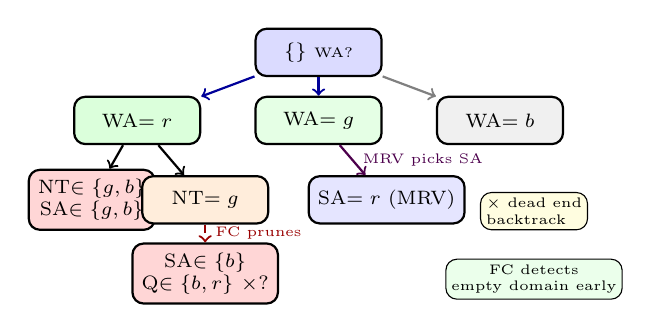
\begin{tikzpicture}[scale=0.72, every node/.style={font=\scriptsize},
  nd/.style={draw, thick, rounded corners, align=center, minimum width=1.6cm, minimum height=0.6cm},
  fail/.style={draw, thick, rounded corners, fill=red!16, align=center, minimum width=1.6cm, minimum height=0.6cm}]
  \node[nd, fill=blue!14] (r) at (4,3.0) {$\{\}$ \tiny WA?};
  \node[nd, fill=green!14] (a) at (0.8,1.8) {WA$=r$};
  \node[nd, fill=green!10] (b) at (4,1.8) {WA$=g$};
  \node[nd, fill=gray!12] (c) at (7.2,1.8) {WA$=b$};
  \node[fail] (a1) at (0,0.4) {NT$\in\{g,b\}$\\SA$\in\{g,b\}$};
  \node[nd, fill=orange!14] (a2) at (2.0,0.4) {NT$=g$};
  \node[fail] (a2f) at (2.0,-0.9) {SA$\in\{b\}$\\Q$\in\{b,r\}$ $\times$?};
  \node[nd, fill=blue!10] (b1) at (5.2,0.4) {SA$=r$ (MRV)};
  \draw[->, thick, blue!60!black] (r) -- (a); \draw[->, thick, blue!60!black] (r) -- (b); \draw[->, thick, gray] (r) -- (c);
  \draw[->, thick] (a) -- (a1); \draw[->, thick] (a) -- (a2);
  \draw[->, thick, red!60!black, dashed] (a2) -- (a2f) node[midway, right, font=\tiny, red!60!black] {FC prunes};
  \draw[->, thick, violet!60!black] (b) -- (b1) node[midway, right, font=\tiny] {MRV picks SA};
  \node[font=\tiny, fill=yellow!12, draw, rounded corners, inner sep=2pt, align=left] at (7.8,0.2) {$\times$ dead end\\backtrack};
  \node[font=\tiny, fill=green!8, draw, rounded corners, inner sep=2pt, align=center] at (7.8,-1.0) {FC detects\\empty domain early};
\end{tikzpicture}
\caption{Backtracking tree with forward checking on Australia (simplified). MRV selects the most constrained variable; FC prunes neighbour domains after each assignment and cuts branches where a domain empties, before deeper recursion.}
\label{fig:backtrack-tree}
\end{figure}

\begin{lstlisting}[language=Python, caption={Backtracking with forward checking and MRV}, label={lst:backtrack}]
def backtrack(assign, domains, csp):
    if len(assign) == len(csp.vars):          # all assigned
        return assign
    var = mrv(assign, domains, csp)           # MRV + degree tie-break
    for val in lcv_order(var, domains, csp):  # least constraining first
        if consistent(var, val, assign, csp):
            new_assign = assign | {var: val}
            new_domains = forward_check(var, val, domains, csp)
            if all(new_domains[v] for v in csp.vars if v not in new_assign):
                result = backtrack(new_assign, new_domains, csp)
                if result is not None:
                    return result
    return None  # backtrack

def forward_check(var, val, domains, csp):
    nd = {v: set(d) for v, d in domains.items()}
    for nb in csp.neighbors[var]:
        if nb not in nd or val not in nd[nb]:
            nd[nb].discard(val)  # binary != constraint
    return nd
\end{lstlisting}

Forward checking is $O(nd)$ per node and already solves many sparse CSPs. When constraints are tighter (e.g.\ Sudoku), we need stronger propagation.

% ============================================================
\section{Arc Consistency and AC-3}
\label{sec:ac3}

\begin{definition}[Arc consistency]
Directed arc $X\to Y$ is \emph{arc-consistent} if for every $x\in D_X$ there exists $y\in D_Y$ with $(x,y)$ satisfying the constraint on $(X,Y)$. A CSP is arc-consistent if all arcs are.
\end{definition}

Enforcing arc consistency can prune without search: if $D_{\mathrm{SA}}=\{r\}$ and $D_{\mathrm{WA}}=\{r,g\}$ with $SA\neq WA$, then $r$ has no support in $D_{SA}$ for WA, so delete $r$ from $D_{WA}$.

AC-3 (Mackworth, 1977) maintains a queue of arcs. Pop $X\to Y$; if \texttt{revise}($X,Y$) deletes a value, enqueue all arcs $Z\to X$ ($Z$ neighbour of $X$) because $X$'s shrinkage may break their support. Terminates when queue empty; result is the maximal arc-consistent subproblem. Complexity $O(ed^3)$ ($e$ arcs, $d$ domain size), $O(ed^2)$ with careful revise.

\begin{figure}[h!]
\centering
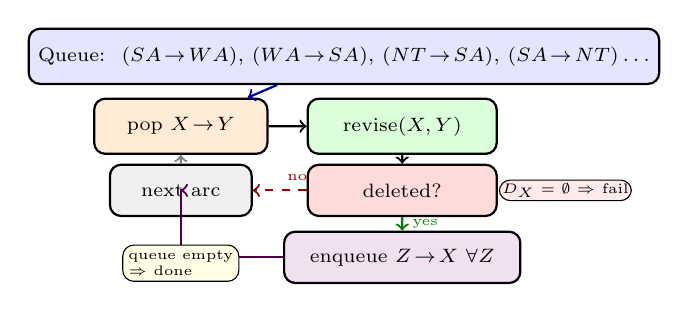
\begin{tikzpicture}[scale=0.74, every node/.style={font=\scriptsize}]
  \node[draw, thick, fill=blue!10, rounded corners, minimum width=7cm, minimum height=0.7cm, align=center] (q) at (4,2.6) {Queue: $\; (SA\!\to\!WA),\, (WA\!\to\!SA),\, (NT\!\to\!SA),\, (SA\!\to\!NT) \dots$};
  \node[draw, thick, fill=orange!16, rounded corners, minimum width=2.2cm, minimum height=0.7cm] (pop) at (1.2,1.4) {pop $X\!\to\!Y$};
  \node[draw, thick, fill=green!14, rounded corners, minimum width=2.4cm, minimum height=0.7cm] (rev) at (5.0,1.4) {revise($X,Y$)};
  \node[draw, thick, fill=red!14, rounded corners, minimum width=2.4cm, minimum height=0.65cm] (del) at (5.0,0.3) {deleted?};
  \node[draw, thick, fill=violet!12, rounded corners, minimum width=3.0cm, minimum height=0.65cm, align=center] (enq) at (5.0,-0.85) {enqueue $Z\!\to\!X$ $\forall Z$};
  \node[draw, thick, fill=gray!12, rounded corners, minimum width=1.8cm, minimum height=0.65cm] (next) at (1.2,0.3) {next arc};
  \draw[->, thick, blue!60!black] (q) -- (pop);
  \draw[->, thick] (pop) -- (rev);
  \draw[->, thick] (rev) -- (del);
  \draw[->, thick, green!50!black] (del) -- node[midway, right, font=\tiny] {yes} (enq);
  \draw[->, thick, red!60!black, dashed] (del) -- ++(-1.8,0) |- (next) node[pos=0.25, above, font=\tiny] {no};
  \draw[->, thick, violet!60!black] (enq) -- ++(-3.8,0) |- (next);
  \draw[->, thick, gray] (next) -- ++(0,0.55) -| (pop);
  \node[font=\tiny, fill=yellow!10, draw, rounded corners, inner sep=2pt, align=left] at (1.2,-0.95) {queue empty\\$\Rightarrow$ done};
  \node[font=\tiny, fill=red!8, draw, rounded corners, inner sep=1pt] at (7.8,0.3) {$D_X=\emptyset\Rightarrow$ fail};
\end{tikzpicture}
\caption{AC-3 queue processing. Each revise may shrink $D_X$; neighbours are re-enqueued only on deletion. Coloured stages show queue $\to$ revise $\to$ enqueue cycle until fixpoint.}
\label{fig:ac3-queue}
\end{figure}

\begin{lstlisting}[language=Python, caption={AC-3 arc consistency}, label={lst:ac3}]
def ac3(domains, csp):
    from collections import deque
    queue = deque((x, y) for x in csp.vars for y in csp.neighbors[x])
    while queue:
        xi, xj = queue.popleft()
        if revise(xi, xj, domains, csp):
            if not domains[xi]:          # empty domain -> unsatisfiable
                return False
            for xk in csp.neighbors[xi]:
                if xk != xj:
                    queue.append((xk, xi))
    return True

def revise(xi, xj, domains, csp):
    revised = False
    for x in list(domains[xi]):
        if not any(csp.satisfies(xi, x, xj, y) for y in domains[xj]):
            domains[xi].remove(x)
            revised = True
    return revised
\end{lstlisting}

\texttt{MAC} (maintaining arc consistency) runs AC-3 after each assignment inside backtracking. Cost per node is higher, but pruning is much stronger---often the best general CSP solver. For tree-structured graphs, AC-3 alone solves without search in $O(nd^2)$ by ordering along the tree; for general graphs search remains exponential worst-case (CSP is NP-complete).

\begin{example}[AC-3 on a chain]
Variables $X,Y,Z\in\{1,2\}$ with $X<Y$, $Y<Z$. Initially all arcs enqueued. Revise $Y\to Z$ deletes $2$ from $D_Y$ (no support $>2$), leaving $D_Y=\{1\}$; this enqueues $X\to Y$. Revise $X\to Y$ deletes $1$ from $D_X$? No---$1$ has support $y=1$? Actually need $x<y$, so $1$ supported by $y$? Wait $D_Y=\{1\}$ after pruning? Check: $Y<Z$ with $Z\in\{1,2\}$ gives $Y\in\{1\}$ only. Then $X<Y$ with $Y=\{1\}$ leaves $D_X=\emptyset$---AC-3 proves unsatisfiability without search. FC after $X=1$ would miss this chain effect.
\end{example}

\begin{remark}[Choosing the engine]
Sparse map-colouring: FC+MRV often suffices. Dense Sudoku or scheduling with AllDifferent: use MAC or a dedicated global propagator (bipartite matching for AllDifferent prunes far more than pairwise $\neq$). Theory guides the trade-off: stronger propagation costs more per node but visits exponentially fewer nodes.
\end{remark}

% ============================================================
\section{Chapter Notes}
Further reading: Russell \& Norvig Ch.~6; Dechter, \emph{Constraint Processing}; Mackworth (1977) on AC-3 and Bessiere on AC-2001. Modern solvers add backjumping, clause learning (for SAT), and global propagators (AllDifferent via matching). Choose FC for sparse, MAC for dense, and exploit structure (cutset, tree decomposition) when the graph is nearly a tree.

% ============================================================
\section{Exercises}
\label{sec:ch04-ex}
\begin{enumerate}[label=E4.\arabic*, leftmargin=*, itemsep=0.75em]
    \item \textbf{Warm-up: formalise.} Model 4-queens as a CSP: give $V$, $D_i$, and all binary constraints. Draw its constraint graph. How many solutions up to symmetry?
    \item \textbf{Heuristics trace.} On Australia with $D_i=\{r,g,b\}$, assign WA$=r$. Apply forward checking, then pick the MRV variable. List pruned domains and explain why degree tie-break favours SA.
    \item \textbf{Arc consistency.} Let $X,Y\in\{1,2,3\}$ with $X<Y$. Show the CSP is not arc-consistent, run AC-3 (queue order $X\!\to\!Y$, $Y\!\to\!X$), give each revise step and final domains. Is the result satisfiable?
    \item \textbf{AC-3 vs.\ forward checking.} Give a 3-variable CSP where FC after $X=a$ leaves domains non-empty but AC-3 detects unsatisfiability. Explain why FC misses it and what extra arc AC-3 revises.
    \item \textbf{MAC complexity.} Prove AC-3 is $O(ed^3)$ and $O(ed^2)$ with an optimized revise that tracks supports. On a tree with $n$ variables, explain why a single AC-3 pass from leaves inward solves the CSP without backtracking.
\end{enumerate}
% End of Chapter 4
